\chapter{Opdrachten}
\label{opdrachten}

\section{Labo-opdracht}
\label{labo-opdracht}

De labo-opdracht omvat het opzetten van ict-infrastructuur op basis van
Linux. We werken in een gevirtualiseerde omgeving en er is een
bijzondere aandacht voor \emph{automatiseren} en \emph{testen}. Je moet
dus in staat zijn de systemen ``from scratch'' op te bouwen met een
minimum aan manuele handelingen. Daarna moet je kunnen aantonen dat deze
systemen voldoen aan de opgelegde specificaties aan de hand van
geautomatiseerde tests en een gedetailleerd testplan en -rapport.

Je kiest aan het begin van het semester één van deze drie opdrachten die je de komende maanden verder uitwerkt.

\begin{itemize}
\item \emph{Small/Medium Enterprise infrastructure:} het opzetten van een bedrijfsnetwerk voor een KMO
\item \emph{High availability:} het opzetten van een robuust webserverplatform
\item \emph{Release Engineering:} het opzetten van een ``build pipeline'' voor de ontwikkeling van webapplicaties
\end{itemize}

Voor het automatiseren van systeembeheertaken maken we altijd gebruik van een
configuration management tool, Ansible. Je krijgt een korte uitleg, maar
het is de bedoeling dat je ook zelf leert werken met Ansible. De
infrastructuur die je bouwt moet telkens volledig ``from scratch''
kunnen worden opgezet zonder manuele tussenkomst.

\subsection{Small/Medium Enterprise infrastructure}
\label{smallmedium-enterprise-infrastructure}

De bedoeling is om een volledig (gevirtualiseerd) netwerkdomein op te
zetten met de enkele typische netwerkdiensten voor een kantooromgeving
(zie Figuur 1).

\begin{figure}[htbp]
\centering
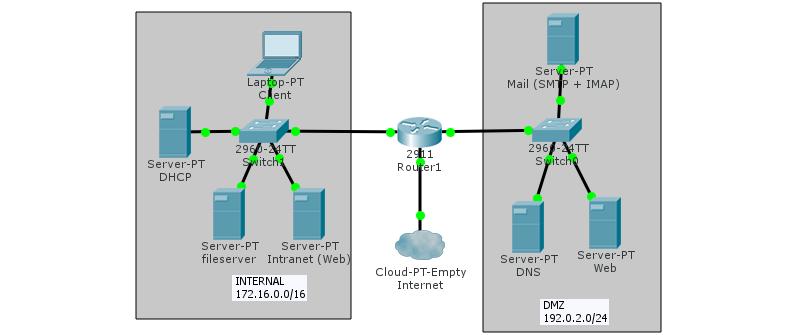
\includegraphics[width=\textwidth]{img/assignment-sme.png}
\caption{Diagram van het op te zetten kantoornetwerk.}
\end{figure}

De opdracht zal in meer detail geformuleerd worden aan de hand van een
reeks deeltaken.

\begin{itemize}
\item LAMP webserver
\item DNS server
\item Fileserver
\item DHCP server
\item Integratie, configuratie router
\end{itemize}

\subsection{High availability}
\label{high-availability}

Hier is het de bedoeling om de infrastructuur op te zetten voor een
grote website die veel webtrafiek moet kunnen verwerken. Dat betekent
dat de webserver ``uit elkaar getrokken'' moet worden en dat
verschillende services op aparte machines moeten komen (zie Figuur 2):

\begin{itemize}
\item Een load-balancer verdeelt netwerktrafiek over verschillende webservers
\item Een cache-systeem zorgt dat niet alle requests leiden tot het opnieuw genereren van een pagina
\item De database-backend komt op een aparte server
\end{itemize}

Bij dit soort opstellingen is het ook essentieel dat de beheerder een
overzicht heeft van de correcte werking van alle componenten. Om dit te
realiseren moet je een monitoring-systeem implementeren met een
dashboard dat een overzicht geeft van het platform.

\begin{figure}[htbp]
\centering
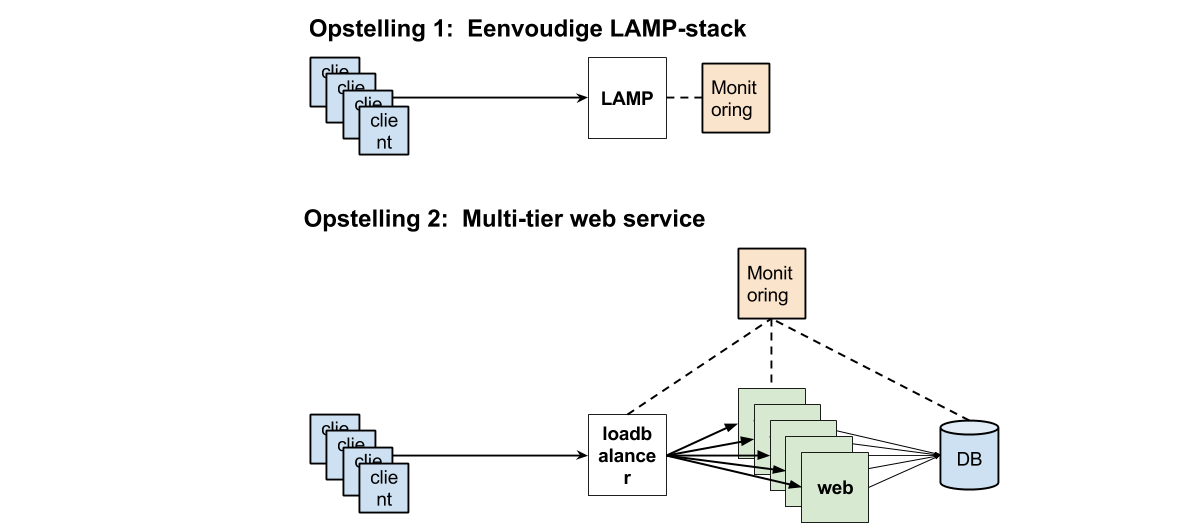
\includegraphics[width=\textwidth]{img/assignment-ha.png}
\caption{Diagram opstelling web server}
\end{figure}

\subsection{Continuous delivery}
\label{continuous-delivery}

In softwarebedrijven of de bedrijven achter de grote websites (type Google, Amazon, Facebook, enz.) is een van de rollen van een systeembeheerder er voor te zorgen dat software-ontwikkelaars zo snel en zo vlot mogelijk nieuwe features in productie kunnen brengen. Deze functie heet ``Release Engineer''. In plaats van grote, ingrijpende releases over langere periodes met veel nieuwe features, streeft men er tegenwoordig naar om kleinere releases te doen aan een hoger tempo (soms zelfs tientallen per dag), met bv. slechts één nieuwe feature of verbetering. Voor deze manier van werken is specifieke infrastructuur nodig en is het nodig een aantal zaken te automatiseren.

De bedoeling van deze opdracht is om een Continuous Delivery ``build pipeline'' te bouwen voor het ontwikkelen van een webapplicatie (je kan zelf een case zoeken, bv. een open source project).

\begin{itemize}
\item De ontwikkelaar werkt op een ``development environment'' in de vorm van een virtuele machine aangestuurd door Vagrant
\item Wanneer de ontwikkelaar code publiceert op de ``master'' branch van een Git repository (bv. op Github) wordt het buildproces opgestart, bestaande uit:

  \begin{itemize}
  \item code-analyse, linting
  \item compilatie
  \item packaging (RPM, .deb)
  \end{itemize}
\item De package wordt uitgerold op een ``QA environment'', een VM op een zelf te kiezen virtualisatieplatform (bv. KVM, OpenNebula) en alle tests (unit, integratie, acceptatie, \ldots{}) worden uitgevoerd
\item Wanneer alle tests slagen, wordt de nieuwe code automatisch uitgerold in de ``productie-omgeving'' op een cloud-platform (bv. Amazon AWS of DigitalOcean).
\end{itemize}

Je moet de hele pipeline kunnen demonstreren. Na een wijziging in de code te pushen moet je (na verloop van tijd) de wijziging op de productieserver kunnen zien.

De VMs die op de verschillende platformen draaien, worden toch zo identiek mogelijk geconfigureerd. Hier bestaan tools voor, bv. Packer.  Je mag ook containers (bv. Docker) gebruiken om je applicatie in te pakken. De build server kan Jenkins zijn, je kan ook kijken naar Travis CI.

\section{Actualiteit}
\label{actualiteit}

Bij elke rol in de ict-sector is het voortdurend bijwerken van je
vakkennis onontbeerlijk om de snelle evolutie in je vakgebied bij te
kunnen benen. In Linux systeembeheer is dat niet anders. Wat ons
vakgebied kenmerkt is een uitgesproken wil om informatie en kennis te
delen. Er is dan ook een schat van informatie te vinden over de meest
recente evoluties via blogs, conferenties waarvan de lezingen op Youtube
of Vimeo gepubliceerd zijn, enz.

De bedoeling van deze taak is aan te tonen dat je deze evoluties ook
opvolgt en probeert toe te passen in de praktijk. Je kan kiezen uit twee
manieren om dit aan te tonen:

\begin{itemize}
\item
  Pas een recentelijk gepubliceerde techniek, tool, \ldots{} uit in het
  kader van de labo-opdracht
\item
  Doe een bijdrage aan een open source project gerelateerd aan de cursus
\end{itemize}

Je mag hier ook tijdens de contacturen aan werken en ook samenwerken met
één of enkele medestudenten is toegelaten. In dat geval moet elke
student individueel de eigen bijdrage kunnen aantonen.

\subsection{Nieuwe technieken
uitproberen}\label{nieuwe-technieken-uitproberen}

Zoals eerder aangegeven, vormen Linux-systeembeheerders een
``community'' waar er veel informatie uitgewisseld wordt. Sommigen
gieten zaken die ze bijleren in een blog-artikel, gaan erover spreken op
conferenties, enz.

De bedoeling hier is om zo'n artikel of lezing toe te passen op de
labo-opdracht. Een paar voorbeelden als inspiratie:

\begin{itemize}
\item
  Hayden (2015) en Davila (2015) beschrijven een manier om
  RHEL/CentOS-systemen te testen op vlak van beveiliging, gebaseerd op
  Ansible. Is het mogelijk dat toe te passen op onze systemen? In het
  artikel gaat het over versie 6, terwijl wij op versie 7.1 zitten. In
  hoeverre kan dit aangepast worden?
\item
  Fail2ban is een Intrusion Prevention System dat een server kan
  beschermen tegen brute-force of denial of service-aanvallen (Sawiyati,
  2014). Kan je dit toepassen op onze servers? Het is uiteraard wel de
  bedoeling dit via Ansible te doen. Dat kan hetzij via een bestaande
  rol (zie Ansible Galaxy), die je zo nodig aanpast, hetzij één die je
  zelf schrijft.
\item
  Secure Shell is de standaard manier om Linux-servers op een veilige
  manier van over het netwerk te beheren. Maar volgens stribika (2015)
  is het mogelijk om \texttt{sshd} nog beter te beveiligen. Kan je dit
  toepassen op onze servers?
\item
  Zoals onze opstelling nu is, zullen wachtwoorden in de
  \texttt{host\_vars} of \texttt{group\_vars} bestanden opgeslagen
  worden. Dit is niet ideaal: we steken onze code in een
  versiebeheersysteem, maar wachtwoorden horen daar met het oog op
  beveiliging helemaal niet in thuis. Ansible heeft hiervoor een
  oplossing:
  \href{https://docs.ansible.com/ansible/playbooks_vault.html}{Ansible
  Vault}. Blanc (2015) beschrijft een methode om het gebruik van Ansible
  Vault zo transparant mogelijk te maken. Kan je het toepassen in onze
  opstelling?
\item
  Johnson (2015) schreef een artikel over het versnellen van Ansible.
  Kloppen zijn aanbevelingen? Kan je dat aantonen, m.a.w. het
  tijdverschil meten tussen de standaardinstellingen en zijn
  aanpassingen?
\end{itemize}

Je kan de blogs waar naar gerefereerd werd in deze voorbeelden opvolgen
(bv. via een RSS reader), hieronder volgen er nog enkele:

\begin{itemize}
\item
  AT Blog: \url{http://www.atcomputing.nl/blog/}
\item
  Cron Weekly newsletter: \url{https://www.cronweekly.com/}
\item
  Erika Heidi: \url{http://erikaheidi.com/blog/}
\item
  Everything Sysadmin (Tom Limoncelli):
  \url{http://everythingsysadmin.com/}
\item
  Everything is a Freaking DNS Problem (Kris Buytaert):
  \url{http://www.krisbuytaert.be/blog/}
\item
  Fedora Magazine: \url{http://fedoramagazine.org/}
\item
  Linux Journal: \url{http://www.linuxjournal.com/}
\item
  Major.io (Major Hayden): \url{https://major.io/}
\item
  ma.ttias.be (Mattias Geniar): \url{https://ma.ttias.be/}
\item
  Planet CentOS: \url{http://planet.centos.org/}
\item
  Runaway Sequence (Aaron Hunter): \url{http://sharknet.us/}
\item
  Standalone Sysadmin (Matt Simmons):
  \url{https://www.standalone-sysadmin.com/blog/}
\item
  SysadminCasts (Justin Weissig): \url{https://sysadmincasts.com/}
\item
  The Geek Stuff: \url{http://www.thegeekstuff.com/}
\end{itemize}

Vond je andere interessante blogs? Geef maar door aan de lector! Andere
bronnen van informatie zijn Youtube of Vimeo (voor presentaties van
conferenties of screencasts), Twitter, enz.

Ben je zelf buiten de opleiding om bezig met Linux? Bespreek met de
lector of je je ervaringen, experimenten, \ldots{} eventueel kan
inbrengen voor deze opdracht.

\subsection{Bijdrage aan een open source
project}\label{bijdrage-aan-een-open-source-project}

Alle tools waar we in de cursus gebruiken zijn open source. Sommige,
zoals Ansible, werden door een softwarebedrijf ontwikkeld die daar een
businessmodel rond gebouwd hebben. Andere werden door enthousiastelingen
in hun vrije tijd ontwikkeld. In elk geval kunnen we gratis gebruik
maken van software van hoge kwaliteit, dankzij de inspanningen van
velen.

Het is passend daar iets voor terug te doen, dus de bedoeling is om een
significante bijdrage te leveren aan een open source project dat
gerelateerd is aan de cursus. Dit kan een kleine bijdrage zijn, maar
voorwaarde is wel dat ze aanvaard is door de auteur(s) van het project.

Je mag hiervoor samenwerken met één of meerdere medestudenten, maar de
individuele bijdrage van elk teamlid moet aantoonbaar zijn (bv. aan de
hand van Git commits).

Enkele mogelijkheden:

\begin{itemize}
\item
  Op Ansible Galaxy zijn veel rollen te vinden die beter kunnen.
  Implementeer een nieuwe feature, zorg er voor dat ze op CentOS 7
  draaien, verbeter fouten, \ldots{} Ook de lector apprecieert hulp bij
  het verder ontwikkelen van zijn Ansible-rollen
  \url{https://galaxy.ansible.com/bertvv/} en
  \url{https://github.com/search?q=user\%3Abertvv+ansible}.
\item
  Schrijf een Ansible rol (waar nog geen alternatief voor CentOS voor
  bestaat) en publiceer die op Ansible Galaxy. Dit doe je best in
  samenwerking met één of meerdere medestudent(en)!
\item
  Pas een techniek die beschreven is voor een andere distributie (CentOS
  6, Debian, Ubuntu, \ldots{}) toe op CentOS 7. In de vorige sectie vind
  je een paar concrete voorbeelden.
\end{itemize}

Andere ideeën zijn ook welkom, bespreek die met de lector. Ook op
Chamilo kan je nog enkele voorstellen vinden.

\section{Troubleshooting}\label{troubleshooting}

Tijdens het semester wordt er een aantal keer een
troubleshooting-oefening gegeven tijdens de contactmomenten.Aanwezigheid
is verplicht, behalve voor TILE-studenten (zie verder).

Bij het begin van de sessie krijg je een virtuele machine waar een
netwerkservice op zou moeten draaien. Door fouten in de configuratie
werkt die echter niet correct. De bedoeling is om op een systematische
en grondige manier de fouten op te sporen en weg te werken en de service
opnieuw beschikbaar te maken over het netwerk. Je maakt daar een
gedetailleerd verslag van dat aan het einde van de les ingediend moet
worden op Chamilo.

\section{Rapportering en
documentatie}\label{rapportering-en-documentatie}

\subsection{Cheat-sheets en
checklists}\label{cheat-sheets-en-checklists}

Wanneer je niet gewend bent om met Linux te werken, dan is het niet
evident om op te zoeken en te onthouden welke commando's je nodig hebt
voor welke taak. Via Google vind je wel vaak een oplossing, maar dat
ligt niet altijd voor de hand. Er zijn bijvoorbeeld recentelijk
substantiële wijzigingen doorgevoerd in de architectuur van de
belangrijkste Linux-distributies waardoor bepaalde commando's (die je
erg vaak tegenkomt bij Googlen) niet meer werken.

Om jezelf te helpen bij het onthouden van de belangrijkste commando's,
is het bijhouden van een cheat-sheet of ``spiekbriefje'' een nuttig
hulpmiddel. Als je een bepaald commando een paar keer bent moeten gaan
opzoeken, dan is het best dat eens te noteren zodat je het in de
toekomst sneller terugvindt en op de duur ook beter onthoudt.

Hetzelfde geldt voor procedures van handelingen die steeds terugkomen.
Bijvoorbeeld, als je wil nagaan of de IP-instellingen van een host
kloppen, gebruik je altijd dezelfde commando's. Wanneer je die telkens
opnieuw moet gaan opzoeken verspil je tijd en het is best mogelijk dat
je zo zaken over het hoofd ziet. Door checklists bij te houden,
verminder je het opzoekwerk en kan je ook vlotter werken (Simmons,
2009).

In je repository vind je onder \texttt{doc/} een bestand
\texttt{cheat-sheet.md} dat een aanzet geeft. Er zijn alvast enkele
nuttige commando's in opgenomen, maar je kan dit zelf aanpassen naar je
eigen smaak. Als het document te groot wordt, kan je het opsplitsen in
verschillende bestanden. Je kan nog meer inspiratie opdoen op deze
Github-repository waar een aantal cheat-sheets en checklists
gepubliceerd zijn: \url{https://github.com/bertvv/cheat-sheets}.

Bij de evaluatie wordt er rekening mee gehouden hoe je deze documenten
hebt bijgehouden in de loop van het jaar (aan de hand van de commit
log).

\subsection{Bloggen}\label{bloggen}

Technische blogs zoals deze die eerder aangehaald werden zijn een meer
en meer voorkomende manier om ervaringen en informatie uit te wisselen
binnen ons vakgebied. Studenten die gaan solliciteren (en ook wie al in
het vak staat) kunnen met een eigen blog aan potentiële werkgevers
aantonen dat ze gepassioneerd zijn door hun vak, bezig zijn met de
laatste technologieën en open staan voor het delen van kennis. Je kan
een eigen blog opstarten en schrijven over wat je in deze cursus (en ook
andere!) leert, zaken die je zelf opgezocht en ondervonden hebt,
\ldots{}

Voorbeeldjes:

\begin{itemize}
\item
  Jürgen Van Meerhaeghe: \url{https://jurgenvm.blogspot.be/}
\item
  Stijn Spanhove: \url{http://www.spanhove.com/blog.htm}
\item
  Thomax Clauwaert: \url{https://ciberth.blogspot.be/}
\item
  Toon Lamberigts en Tomas Vercautter: \url{https://t0t0.github.io/}
\end{itemize}

Dit is vrijblijvend, maar heeft wel een positieve invloed op je
examencijfer.

